% Introduction to SNR optimisation in PyCBC Live

The optimal methods for optimising signal-to-noise ratio in PyCBC Live was researched and improved multiple times across the course of the PhD. These changes are being written up in the PyCBC Live fourth observing run methods paper. ADD A BIT OF INFORMATION

\section{\label{7:sec:introduction}Introduction}

% % Background and Context
% Big Picture: Start by placing the topic in a broader scientific or academic context. Why is this field of study important?
% Specific Focus: Narrow down to the specific problem or area your paper/chapter will address.

As described in chapters~\ref{chapter:5-pycbc-live} and~\ref{chapter:6-earlywarning} the PyCBC Live search pipeline (among others) is responsible for detecting and producing accurate sky maps of \gwadj signals in low-latency. Search pipeline events are uploaded to the Gravitational-Wave Candidate Event Database~\cite{ligo_gracedb:2024} (GraceDB) from which a \textit{preferred event} is chosen to send a GCN Circular~\cite{gcn_circulars:2024} (a rapid astronomical bulletin submitted by and distributed to astronomy community members worldwide). The preferred event is chosen based on a listed selection criterion. These rules are taken verbatim from~\cite{gracedb_superevent_selection}:

When multiple online searches report events at the same time, the preferred event is decided by applying the following rules, in order:
%
\begin{itemize}
    \item A publishable event, meeting the public alert threshold, is given preference over one that does not meet the threshold.
    \item An event from CBC searches is preferred over an event from unmodeled Burst searches (see Searches for details on search pipelines).
    \item In the case of multiple CBC events, three-interferometer events are preferred over two-interferometer events, and two-interferometer events are preferred over single-interferometer events.
    \item In the case of multiple CBC events with the same number of participating interferometers, the event with the highest SNR is preferred. The SNR is used to select the preferred event among CBC candidates because higher SNR implies better sky location and parameter estimates from low-latency searches. In the case of multiple Burst events, the event with the lowest FAR is preferred.
\end{itemize}
%
The PyCBC Live search is a CBC search and when analysing the same number of interferometers as other CBC searches there is a tie-breaker for preferred event dependent on the SNR of the event.

% 2. Motivation and Relevance
% Why This Topic?: Explain why the topic of your paper or chapter matters. What are the practical, scientific, or theoretical reasons that make it worth investigating?
% Gap in Knowledge: Identify any gaps or unresolved issues in the current literature that your work will address.
It is clear from these set of rules that to become the preferred event we must upload the event with the highest SNR. This is where the PyCBC Live SNR optimiser becomes relevant. We construct our template bank with a minimum match of $0.97$, allowing up to a $3\%$ SNR loss for any event. If we want to maximise the SNR of our event we must perform a finer search over the template bank parameter space around the initially found template to recover that potentially lost $3\%$.

% 3. Objectives and Research Questions
% Main Goals: Clearly state the primary objectives of the chapter or paper. What do you aim to achieve or contribute?
% Research Questions: If applicable, list specific research questions or hypotheses that guide your work.
The SNR optimiser uses optimisation algorithms which tune input parameters (template parameters) to maximise (or minimise) an output (network SNR). There are a number of different optimisation algorithms operating under different mathematical optimisation techniques all of which have hyperparameters which can be tuned to the problem space to optimise optimiser performance---both output value and computational time.

We detail the investigation into an optimal optimisation algorithm for PyCBC Live along with the tuning of the hyperparameters for this optimisation algorithm, how these algorithms were tested and the results of using the SNR optimiser on a number of PyCBC Live events.




% Goals: State what you aim to cover in this chapter (history, methods, results, and implementation).

In this chapter we begin by discussing the need for the SNR optimiser.

Then we discuss the historical background for the snr optimiser, the need for it and the initial configuration.

Then we move on to the research performed by me to initially select optimal hyperparameters for the optimiser. How we did this, what did we test, which optimisers and event type (BBH, BNS, NSBH). DE, SHGO, the other one?

Then we look at PySwarms.

Then we look at some results.

Then we look at some final research into chirp times and astrophysical bounds, initial point in the swarm and potentially template bank initial points.

Then we discuss future improvements to this programme.

\section{\label{7:sec:optimising_snr_in_low_latency}Optimising SNR in low-latency}

The PyCBC Live search will matched filter the entire template bank with the data ring buffer every analysis stride (see chapter~\ref{chapter:5-pycbc-live} for greater detail). The matched filter will produce SNR triggers when any template has been found with a matched filter above an SNR of $4.5$. The PyCBC Live search will then pass these triggers to the ranking statistic, taking into account any signal-consistency test values or other ranking statistic components, to find the most significant coincident set of triggers. After the uploading of an event to GraceDB, the PyCBC Live search will spawn a subprocess and the PyCBC programme \texttt{pycbc\_optimize\_snr} is initialised. This programme takes the \gwadj data and is given the event template parameters to run a finer search over the parameter space specifically optimising for the network SNR. This finer search is performed not using a template bank approach but with an optimisation function, a process that finds the `best' possible solution by maximising for a particular objective given input parameters that can be tuned. For PyCBC Live the objective being maximised is the network SNR and the tunable input parameters are the template bank parameters: primary component mass $m_{1}$, secondary component mass $m_{2}$, primary spin z-component $s_{1z}$ and, secondary spin z-component $s_{2z}$. Boundaries are applied to the input parameters which are calculated using the initial event parameter values.

We run this SNR optimisation to become the preferred event for the GraceDB `superevent' (the \gwadj signal each pipeline event has observed). An example for a recent \gwadj signal (S240924a~\cite{superevent_S240924a}) can be seen in figure~\ref{7:fig:gracedb_pref_event}.
%
\begin{figure}
    \centering
    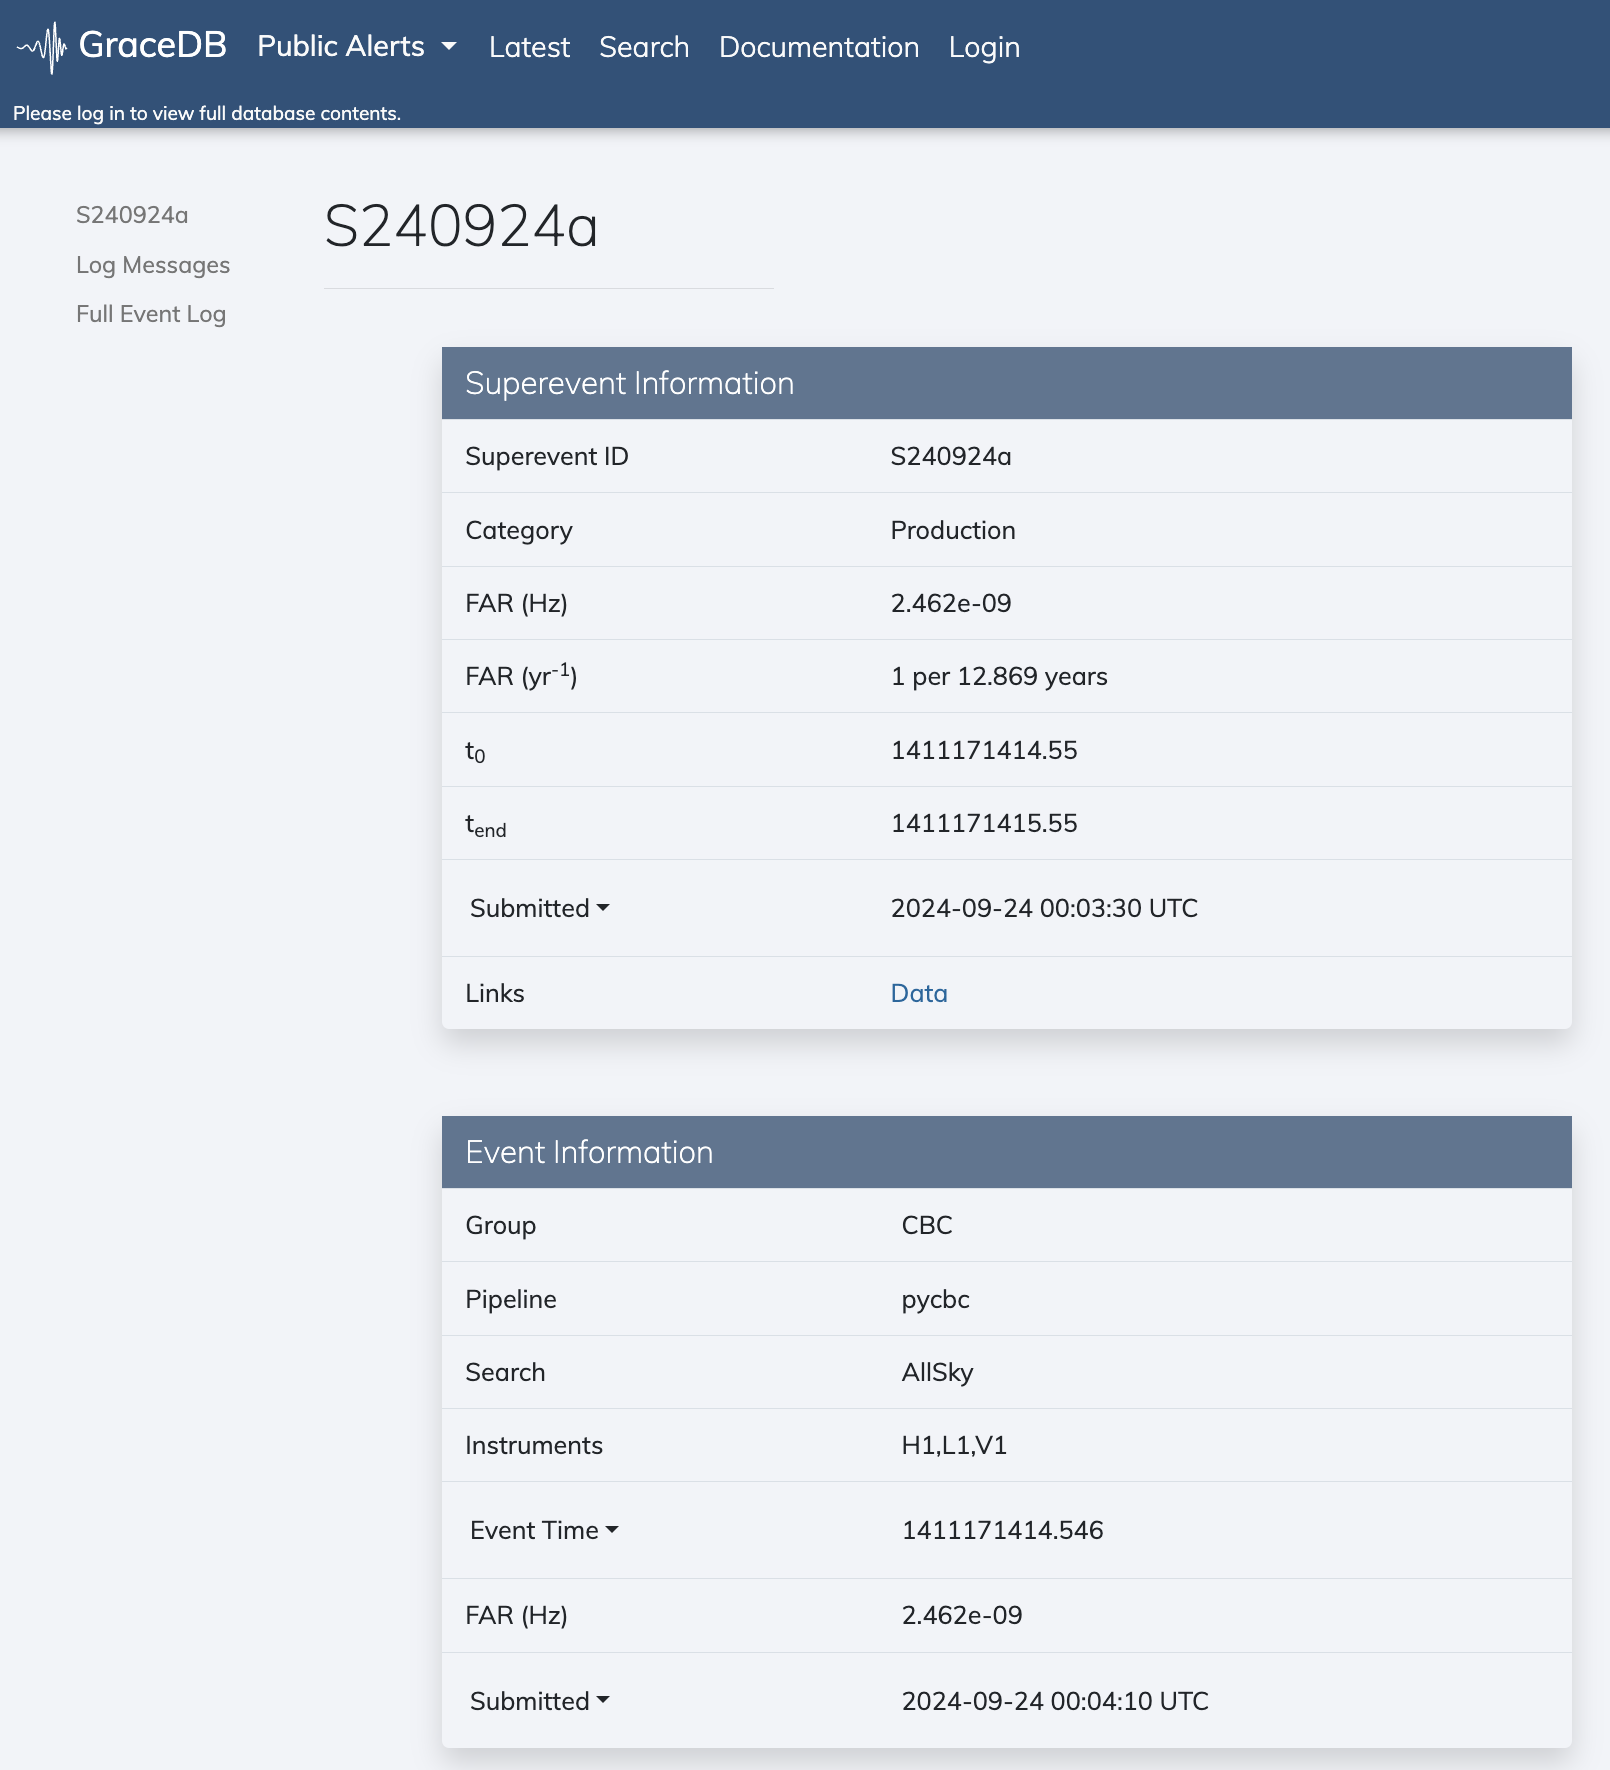
\includegraphics[width=1.0\linewidth]{images/7_snr_optimiser/gracedb_public_snr_optimiser.png}
    \caption{The public webpage for the superevent \gwadj signal observed on the 24$^{\text{th}}$ September 2024, S240924a~\cite{superevent_S240924a}. The preferred search pipeline for this event can be seen in the table titled `Event Information', where it can be seen that a PyCBC Live is the preferred event.}
    \label{7:fig:gracedb_pref_event}
\end{figure}
%
When all pipelines pass the public alert threshold and use the same number of interferometers the tie for preferred event is broken by the SNR of the event. For S240924a we can see the PyCBC event (which was the preferred event) was an SNR optimised event, indicated by the label `SNR\_OPTIMIZED' in figure~\ref{7:fig:gracedb_snr_optimizer}.
%
\begin{figure}
    \centering
    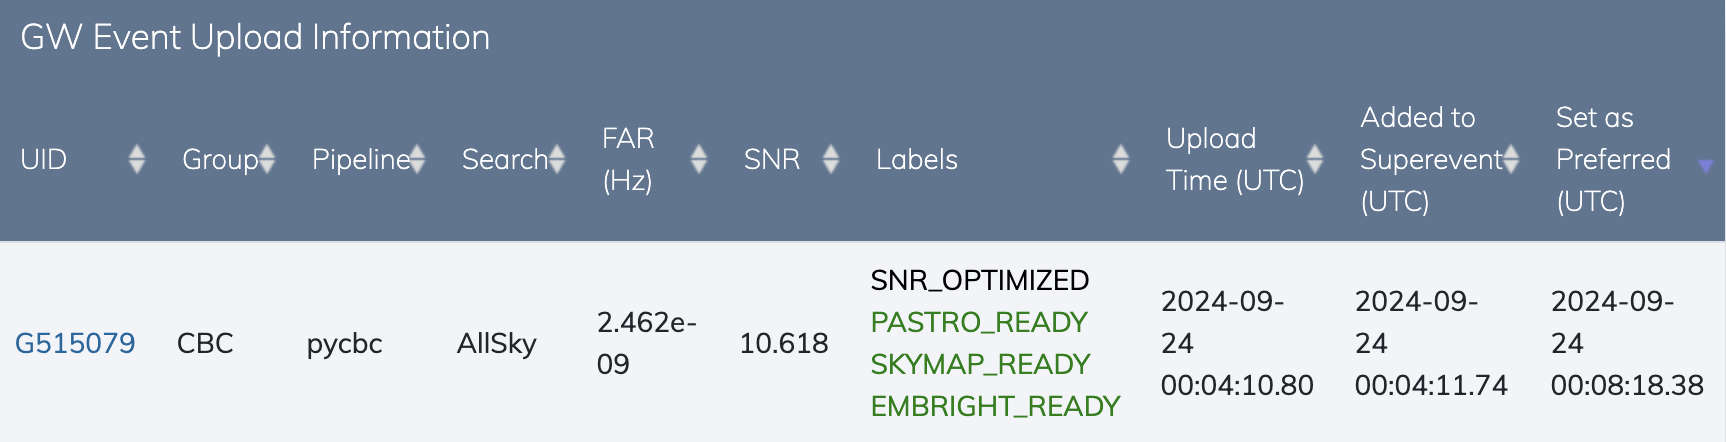
\includegraphics[width=1.0\linewidth]{images/7_snr_optimiser/gracedb_pycbc_pref_event.png}
    \caption{The preferred event for the superevent S240924a~\cite{superevent_S240924a} identified by the PyCBC Live search pipeline (among others). This PyCBC Live event was created by the SNR optimiser.}
    \label{7:fig:gracedb_snr_optimizer}
\end{figure}
%

The original PyCBC SNR optimiser was introduced during the second half of the third observing run to improve the sky maps that are generated by PyCBC Live using the SciPy~\cite{SciPy:2020} optimiser \texttt{differential evolution}~\cite{DE:1997}. Examples noted in the original Github pull request~\cite{pycbc_pull_request_2659} see increases in network SNR from $9.818$ to $10.149$, an increase of $3.6\%$.

Optimisation algorithms can generally be categorised into two main types based on their approach to searching the parameter space: population-based algorithms and single-solution algorithms. Population-based algorithms initialise a set of candidate solutions (a population) and explore the parameters space iteratively using interactions between the candidates to locate the optimal solution. Single-solution algorithms use a single candidate point that is iteratively improved based on some criteria. Only population-based algorithms have been considered for the PyCBC Live SNR optimiser for their computational efficiency in parallelised computing environments where the network SNR of each point can be computed in parallel using a large number of computing cores. These population-based algorithms all follow the same general steps in optimisation.
%
\begin{enumerate}
    \item Initialise a population of size $N$ with random parameter values
    \item Evaluate the network SNR of the point
    \item Adjust each point in the population using the base optimisation algorithm
    \item Re-evaluate the network SNR of each point
    \item Keep points with greater network SNR
    \item Repeat until the number of max iterations has been reacher \textbf{OR} the population has converged on a point
    \item Output the optimised template solution
\end{enumerate}
%
These instructions can vary slightly for optimisation algorithms and we will explore these differences as well as the point adjusting algorithms in the following sections.

\subsection{\label{7:sec:original_bounds}Parameter bounds}

The optimiser will be passed the template parameters of the event that triggers the SNR optimisation. From these parameters the \textit{bounds} are defined. These bounds represent the minimum or maximum value that the optimiser can explore for a specific parameter, preventing it from searching areas we do not want it to search.

The mass parameter bounds are created by converting $m_{1}$ and $m_{2}$ into chirp mass, $\mathcal{M}$, and symmetric mass ratio, $\eta$; this combination leads to a more physically meaningful difference in waveform when changed. The $\mathcal{M}$ bounds are calculated
%
\begin{align}
    \mathcal{M}_{\min} &= 
    \begin{cases}
        \mathcal{M} \cdot \left(1 - \frac{\mathcal{M}}{50.0}\right) & \text{if } \mathcal{M} \cdot \left(1 - \frac{\mathcal{M}}{50.0}\right) \geq 1 \\
        1 & \text{if } \mathcal{M} \cdot \left(1 - \frac{\mathcal{M}}{50.0}\right) < 1
    \end{cases} \\
    \mathcal{M}_{\max} &= 
    \begin{cases}
        \mathcal{M} \cdot \left(1 + \frac{\mathcal{M}}{50.0}\right) & \text{if } \mathcal{M} \cdot \left(1 + \frac{\mathcal{M}}{50.0}\right) \leq 80 \\
        80 & \text{if } \mathcal{M} \cdot \left(1 + \frac{\mathcal{M}}{50.0}\right) > 80.
    \end{cases}
\end{align}
%
The remaining parameter bounds are set to
%
\begin{align}
    0.01 &\ge \eta \ge 0.2499, \\
    -0.9 &\ge s_{1z} \ge 0.9, \\
    -0.9 &\ge s_{2z} \ge 0.9, \\
\end{align}
%
independent of initial event parameters.

Upon creating an instance of the optimiser a population of candidate solutions is randomly initialised. The first hyperparameter we consider is population size, $N$, determining the number of points in the population. Each point is a 4-dimensional vector, $\textbf{x}_{i}$, given a random value for each parameter inside the bounds, $\textbf{x}_{i} = (\mathcal{M}_{i}, \eta_{i}, s_{1z, i}, s_{2z, i}$), this is our initial population, $\textbf{x}_{N}$.

\subsection{\label{7:sec:original_de}The original SNR optimiser}

The differential evolution optimiser is a stochastic, population-based algorithm that iteratively 'mutates' the population to improve individual SNRs. We can visualise the algorithm as a process similar to natural evolution, where, in each iteration, individuals undergo genetic variation through mutation. This combines features from other individuals to create new trial candidates. Just as nature favours the survival of the fittest, the algorithm evaluates the performance of these trial candidates and retains those that exhibit greater SNR, gradually steering the population towards the optimal solution.

When using differential evolution, we have four key hyperparameters:
%
\begin{itemize}
    \item \textbf{Population size, \( N \)}: Determines how many individuals are in the population.
    \item \textbf{Maximum number of iterations}: Sets how long the algorithm runs, i.e., the maximum number of generations.
    \item \textbf{Mutation factor, \( F \)}: Controls the magnitude of mutation and influences how much individuals are altered by the mutation vectors.
    \item \textbf{Recombination constant, \( R \)}: Also known as the crossover probability, it determines the likelihood that a trial candidate takes parameters from the mutation vector instead of the original individual.
\end{itemize}
%
Another hyperparameter, which we do not tune, is the number of processes that are spawned to run the algorithm in parallel. This is set to ``as many as possible'' when running with PyCBC Live. We use the \texttt{best1bin} strategy for generating new individuals.

The algorithm begins by spawning a population of individuals with initial parameter values within the defined bounds. The network SNR for each individual is calculated, and the individual with the highest SNR, \( \mathbf{x}_{best} \), is identified. Next, a set of mutation vectors are created,
%
\begin{equation}
    \mathbf{v}_i = \mathbf{x}_{best} + F \cdot (\mathbf{x}_{r1} - \mathbf{x}_{r2}),
\end{equation}
%
where \( \mathbf{x}_{r1} \) and \( \mathbf{x}_{r2} \) are distinct random individuals from the population. A trial candidate, \( u_i \), is created by combining the mutation vector \( \mathbf{v}_i \) with the target individual \( \mathbf{x}_i \), according to the rule
%
\begin{equation}
    u_{ij} = 
    \begin{cases} 
    v_{i,j} & \text{if } r_j < R \\ 
    x_{i,j} & \text{otherwise}.
    \end{cases}
\end{equation}
%
Here, \( u_{ij} \) is the \( j \)-th parameter of the trial candidate \( u_i \), \( v_{ij} \) is the \( j \)-th parameter of the mutation vector \( v_i \), and \( x_{ij} \) is the \( j \)-th parameter of the target individual \( x_i \). \( r_j \) is generated uniformly in the interval \([0, 1)\). If \( r_j < R \), the mutation vector value is used; otherwise, the original target individual's value is retained. One exception is that the final parameter (4th) \textbf{always} takes its value from the mutation vector, ensuring that no individual remains completely unchanged in the new population.

Once all trial candidates have been generated, their network SNRs are calculated and compare to the target individual SNR. If a trial candidate has a higher network SNR than the original target individual, it replaces the target. If not, the trial candidate is discarded. The process of creating mutation vectors and generating trial candidates is repeated until the maximum number of iterations is reached or another stopping criterion is satisfied.

\subsection{\label{7:sec:de_hyperparameter_tuning}Tuning hyperparameters}

The initial research into the PyCBC Live SNR optimiser involved tuning the four hyperparameters for the differential evolution optimiser:
%
\begin{itemize}
    \item Population size
    \item Maximum number of iterations
    \item Mutation factor
    \item Recombination factor
\end{itemize}
%
a balance must be struck between SNR and computing time. To maximise network SNR we would use larger population sizes, more iterations, higher mutation factors and a lower recombination rate but this will widen the effective search radius and increase the amount of time taken to find an optimised value.

As shown previously the original values for the hyperparameters were able to recover the $3\%$ missing SNR from any template mismatch therefore, we chose to tune hyperparameters to reduce the time to run the programme. The computing time is directly related to both the population size and maximum number of iterations, which had initial values $N = 200$ and $\texttt{maxiter} = 100$. Using a simple grid search over these two hyperparameters for a number of events we were able to maintain the SNR recovery while reducing the computing time by ${\sim}25\%$ on average using $N = 100$ and $\texttt{maxiter} = 50$. These were the first set of improvements for the PyCBC Live SNR optimiser.




\section{\label{7:sec:exploring_alt_opts}Exploring alternate optimisation algorithms}

After tuning the differential evolution optimisation algorithm we began to investigate other optimisation algorithms that could be used to greater success for the PyCBC Live problem space. The SciPy package has an entire module dedicated to optimisers, \texttt{scipy.optimize}, and after testing we discovered that differential evolution was still the best suited for the job of optimising SNR in PyCBC Live.

Looking outside of SciPy we identified the particle swarm optimisation (PSO) algorithm~\cite{pso:1995} as a candidate for the PyCBC Live SNR optimiser. This algorithm was being used for \gwadj searches as shown by~\cite{pso_search_1:2018} and more recently~\cite{pso_search_2:2023}. This made it a good candidate for optimising network SNR in PyCBC Live.



\subsection{\label{7:sec:pso}The optimal algorithm---Particle Swarm Optimisation}

We can describe the particle swarm optimisation (PSO) algorithm similar to how we previously described the differential evolution algorithm. PSO has the hyperparameters:
%
\begin{itemize}
    \item Number of particles, $N$
    \item Maximum number of iterations, $T$
    \item Inertia weight: weight next iteration velocity based on the previous iteration velocity, $w$
    \item Personal learning rate, $c_{1}$
    \item Social learning rate, $c_{2}$
\end{itemize}
%
the number of particles and maxmimum number of iterations are identical to the differential evolution hyperparameters. The personal and social learning rates can be considered as acceleration coefficients of the particle.

Once again, we are maximising the network SNR of the PyCBC Live event, adjusting the template parameters ($m_{1}$, $m_{2}$, $s_{1z}$ and $s_{2z}$) to find the optimal values to give the maximum network SNR. PSO will initialise a ``swarm'' of particles, each with a unique combination of template parameters which can be considered the position of the particle in the parameter space, $\mathbf{x}_{i}$, the particle will also be given a random velocity, $\mathbf{v}_{i}$. The network SNR of each particle is calculated and the personal best of every particle is set, $\textbf{p}_{i}$ (as this is the only position the particle has occupied). From the swarm the global best position is determine, $\textbf{g}$.

Next, we update the velocity of each particle
%
\begin{equation}
    v_{i(t+1)} = w \cdot \mathbf{v}_i(t) + c_1 \cdot r_1 \cdot (\mathbf{p}_i - \mathbf{x}_i(t)) + c_2 \cdot r_2 \cdot (\mathbf{g} - \mathbf{x}_i(t)),
    \label{7:eq:pso_velocity_equation}
\end{equation}
%
where $w$ is the inertial velocity of the particle, $c_{1}$ is the personal learning rate, $c_{2}$ is the social learning rate, $r_{1}$ and $r_{2}$ are random numbers uniformly distributed in $\left[0, 1\right]$, $\textbf{p}_{i}$ is the personal best position of particle $i$ and $\textbf{g}$ is the global best position of the swarm. We can break equation~\ref{7:eq:pso_velocity_equation} down into three distinct contributions to the velocity of the particle at iteration $t + 1$: $w \cdot \textbf{v}_{i}(t)$, how much weight is placed on the previous velocity of the particle, adjusted using the inertia weight hyperparameter; $c_{1} \cdot r_{1} \cdot \left(\textbf{p}_{i} - \textbf{x}_{i}(t)\right)$, how strongly the particle pulls toward its personal best, adjusted using the personal learning weight hyperparameter; $c_{2} \cdot r_{2} \cdot \left(\textbf{g} - \textbf{x}_{i}(t)\right)$, how strongly the particle pulls toward the global best, adjusted using the social learning weight hyperparameter.

After the velocity of each particle is calculated the particle positions are updated
%
\begin{equation}
    \mathbf{x}_i(t+1) = \mathbf{x}_i(t) + \mathbf{v}_i(t+1),
\end{equation}
%
and the network SNR of each particle is calculated again. The particle personal bests and the global best are re-evaluated and updated if they have changed and the iterative process repeats. Upon reaching the number of iterations or if there is convergence in the network SNR value, the algorithm is stopped and the optimal template parameter values are returned which maximise the network SNR.

Upon testing the particle swarm optimisation algorithm was found to be superior to the differential evolution algorithm in both SNR recovery and computing time.

\subsection{\label{7:sec:additional-improvements}Additional improvements}

The PyCBC programme \texttt{pycbc\_optimize\_snr} has been under irregular but constant development to improve the functionality. There are a number of small improvements to the programme which can help improve the computing time and maximum SNR found.

\subsubsection{Initial point in the population}

The SNR optimiser can miss the maximum SNR of the parameter space if it is not searched with a fine enough set of particles. Not only can the maximum point be missed but the maximum can be found below the SNR recovered by the initial PyCBC Live event. To prevent this we can set a floor on the optimiser SNR by including our initial guess into the initial swarm (or population). Including this initial template into the swarm will set the best position allowing for a faster convergence on the maximum SNR.

\subsubsection{Astrophysical spin bounds}

The bounds described in section~\ref{7:sec:original_bounds} are very general and cover a wide parameters space. The PyCBC Live search is capable of detecting \gwadj signals from binary black hole, binary neutron star and, neutron star - black holes. We know that neutron stars have a physical limit on spin~\cite{Harry_Lundgren:2012} therefore we can impose more astrophysically informed spin bounds on objects with masses consistent with neutron stars
%
\begin{align}
    \text{spin bounds} &= 
    \begin{cases} 
        -0.4 - 0.4 & \text{if } \text{max mass} < 3 \, M_{\odot}, \\
        -0.9 - 0.9 & \text{if } \text{max mass} > 3 \, M_{\odot},
    \end{cases} 
\end{align}
%
it is important to impose the condition dependent on the maximum mass the optimiser is allowed to search over. If the optimiser is allowed to assign masses to particles greater than the upper mass limit on neutron stars then we have to let the spin vary by up to the black hole spin bounds because the optimal template could be in this region even if the initial template (from which the bounds are calculated) isn't.

\subsubsection{Chirp time boundaries}

Another improvement made to the parameter bounds is determining the $\mathcal{M}$ bounds using a constant chirp time window. We define the chirp time as the time between the start of the signal (at some define lower frequency, $f_{L}$) and the peak frequency prior to the merger
%
\begin{equation}
    \tau_0 = A_{0}\left(\mathcal{M}\right)^{-5/3}.
\end{equation}
%
where
%
\begin{equation}
    A_{0} = \frac{5}{256 \left(pi f_{L}\right)^{8/3}}.
\end{equation}
%
The chirp time to Newtonian order, $\tau_{0}$, depends only on the two masses, $m_{1}$ and $m_{2}$~\cite{Cokelaer:2007}. By using a chirp time window we can search the $\mathcal{M}$ parameter space for signals that look far more physically similar than if we were just changing $\mathcal{M}$ itself.

A higher mass \gwadj event will merge at lower frequencies and therefore have a shorter chirp time. To calculate the $\mathcal{M}$ bounds we first calculate the chirp time of the initial event, then we subtract the constant chirp time window ($2$ seconds in PyCBC Live) and convert back to $\mathcal{M}$ to find the maximum $\mathcal{M}$ bound and add the window and convert to find the minimum $\mathcal{M}$ bound.

We also improve the $\eta$ bounds by imposing a minimum mass of any component object $\text{min}(m) = 0.99$ and calculating the maximum mass of $m_{1}$ using the maximum $\mathcal{M}$. Using this we can calculate the \textit{minimum} value of $\eta$, again by using the minimum mass of any component and the maximum mass of $m_{1}$. Then using the same maximum $\eta$ previously defined we are able to define the upper mass bound on $m_{2}$.

These changes to the parameter bound calculation give us the boundaries for $\mathcal{M}$ and $\eta$ as
%
\begin{align}
    \left(\frac{A_{0}}{\tau_{0} + 2.0}\right)^{\frac{3}{5}} &\ge \mathcal{M} \ge \left(\frac{A_{0}}{\tau_{0} - 2.0}\right)^{\frac{3}{5}}, \\[10pt]
    \frac{\text{max}(m_{1}) \cdot 0.99}{(\text{max}(m_{1}) + 0.99)^{2}} &\ge \eta \ge 0.2499,
\end{align}
%
which allow for less time to be wasted in computing regions of the parameter space which we know will not contain the maximum point.

\section{\label{7:sec:results}Results}
% Performance Gains: Present quantitative results showing how the optimiser improved the SNR detection in PyCBC Live.
% Comparison with Previous Methods: Compare the final results with the performance of earlier non-optimised or less-optimised techniques.
% Error Reduction and Accuracy: Discuss the improvement in false positive rates or computational efficiency.
% Impact on Real-time Detection: How did the optimiser improve the real-time performance of the detection pipeline?



% How many events were PyCBC preferred SNR optimised
% How many of these events wouldn't have been preferred if we didn't have the SNR optimiser
% Average SNR % increase + Computing time
% Histograms of these




\section{\label{7:sec:discussion}Discussion}
% Limitations: Discuss any limitations of the current optimiser (e.g., computational bottlenecks, situations where the optimisation struggles).
% Broader Impact: How does this optimisation contribute to the broader field of gravitational wave detection?
% Future Work: Mention potential improvements or future research directions that could enhance the SNR optimisation process further.



\section{\label{7:sec:conclusion}Conclusion and future improvements}
% Summary: Recap the importance of the SNR optimiser and its role in improving gravitational wave detection.
% Final Thoughts: Reflect on the significance of this work in the context of the PyCBC pipeline and real-time gravitational wave detection efforts.

\subsubsection{Template bank initial population positions}

% Other optimisers
%  With the vast growth of ML during this PhD you can do a million things
% GPU acceleration
% 





